\chapter{Implementation details}
\section{Architecture}
here goes the uml
\begin{figure*}[h]
\centering
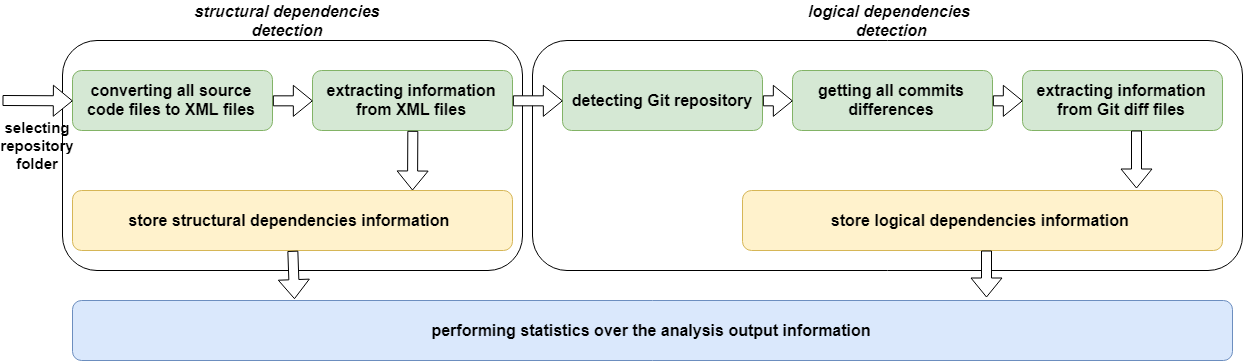
\includegraphics[width=\textwidth]{fig3.png}
\caption{Processing phases}
\label{fig:fig3}
\end{figure*}

\section{Extracting software dependencies}
\subsection{srcML}
SrcML is an open source tool that converts in an XML format C/C\#/Cpp/Java source code. \cite{srcml1}\\
All the original source code files are kept and the corresponding XML files are created. Each source code file is converted in a single XML document.\\
 The srcML toolkit includes \textbf{source-to-srcML} and \textbf{srcML-to-source} translators:
\begin{itemize}
  \item source-to-srcML : is responsable for source code to XML conversion.
  \item srcML-to-source : is responsable for XML to source code conversion, so that the original source code document can be recreated from the srcML XML file.
\end{itemize}

The srcML XML contains of all text from the source code file and XML tags. The file contains all the syntactic structures from the code (e.g., classes, structures, functions, function call, destructors, methods, if statements, for statements, switch statements, etc.).\cite{srcml2}
An example of the XML representation can be found in .
\subsection{XML parser}


\section{Extracting logical dependencies}
tbd\\
The second step of the analysis is to extract logical dependencies from the versioning system. The versioning system contains the long-term change historyofeveryfile.Changes can be made by many individuals over the years.\\ 
Changes include the creation and deletion of files as well as edits to their contents. Each change (this can include changes in multiple files) made by an individual at certain point of time is contained into a revision\cite{ct7}. All the revisions are stored in the versioning system cronologicaly and each revision has a parent revision. 
\\ The parent revision is the revision from which development began, the only exeption to this rule is the first revision which has no parent revision.We will take into consideration only revisions that have a parent revision since the first revision can include source code files that are already in development (migration from one versioning system to another) and this can introduce reduntant logical links . We also will take into consideration only revisions that contain changes in at least one file with .java extension since our main focus is finding classes that change together that can only be contained in .java and .cpp files \cite{ct8} .
\\ The tool looks through the repository and gets all the existing revisions, for each revision a differences file will be made . The differences file will contain all the changes from all the files merged . Before making the differences file, the revision shall fulfill all the conditions mentioned above. In addition each file will be saved with the number of .java and .cpp files changed in his name. In this way it will be more easy to filter the revisions differences files by the number of files changed. Finally after all the differences files are stored , all the files are parsed and logical dependencies are build. The logical dependencies are splitted into three categories : dependencies found in revisions with less than 5 files changed, dependencies found in revisions with more than 5 files changed but less than 20 and dependencies found in revisions with more than 20 files changed. Also dependencies found with only comments change where not taken in to consideration (classA and classB change together but the only change found is in comments).

\section{Saving and restoring the information processed}
tbd